\section{Vistas on ontologies}\label{vistas}
\epigraph{¿No basta un solo término repetido para desbaratar y confundir la serie del tiempo? ¿Los fervorosos que se entregan a una línea de Shakespeare no son, literalmente, Shakespeare?}{\cite{confutacion}}
Looking at our \autoref{sec_coins} it's surprising how mathematically consistent Borges' universe becomes when it is described through category theory. As we already said, this has to be regarded as an experiment, a literary \emph{divertissement}, and a test-bench for our main claim, that as abstract as it may seem ontology has a quantitative content.

There is clearly no point to just analyse Borges' literary work: we can go further. The present section has this purpose, while sketching somelong term goals our work can aspire to become. We begin with a more academic discussion of classical idealism \emph{à la} Berkeley; of course, in light of our \autoref{incendiata}, this can still be linked to Tl\"on's universe, as Borges has always been fascinated by, and mocked, classical idealism (see \cite{confutacion}).

To this, it follows a more wide-ranging discourse; surely a less substantiated one, but we aim at laying a foundation for future work, ours or others', in a research track that we feel is fertile and promising.
\subsection{Answers to the idealist}\label{berkelei}
Let us reconsider \autoref{bla}; although in passing, we mentioned famous Berkeley's view of perception as a bundle of stimulation incapable to cohere. Let's say clearly that endeavouring on such a wide ground as classical idealism isn't the purpose of our work; yet, in his novel Borges regards Tl\"on's language and philosophy as a concrete realisation of Berkeley's theory of knowledge. We thus find natural to explore such link with a classical piece of philosophy, as far as it can be taken.

Once accepted that there are nine coins, Berkeleyan instantaneist cuts every existence $p(g,c,d) < (\top,1)$ at the ``purely false'' value, so that $\forall c.\forall d.\sum_u p(u,c,d) = (\bot,1)$. They find our notion of admissibility for a configuration of coins untenable, as only what exists completely deserves to \emph{be}. On this side of the barricade, we find instantaneism untenable: what exists \emph{completely} (or rather, what \emph{exists} completely)? Equally untenable is idealism, the belief that whatever lacks a percipient conscience must suddenly disappear in thin air (thus, God must exist).

However, as strange and counterintuitive as it may seem, instantaneism and idealism have their point on Tl\"on:\footnote{Somehow, \cite{tlonEN} isn't far from an artificial world built in order to mock idealism; cf. also \cite{borges1997otras} and the famous essay \cite{confutacion} therein.} we should then be able to find a tenable justification for them, from within topos theory. Surely, we aim at doing so ``making no pact with the impostor Jesus Christ''.

As we have seen throughout the entire work, in the internal language of a topos a proposition $p$ takes its truth values in a much wider range of possibilities where instead of a yes-no, all-nothing opposition, existence gives way to a more nuanced notion that can be (in)valid with a certain strength $t : I$. The language we introduced so far precisely quantifies how much Berkeley's ``cut'' above is a blunt one, easily falsifiable (to say the least) even on Tl\"on. Instantaneism arises forgetting topology and order on $I$ (cf. \autoref{}), and idealism from quotienting one of the copy $I\times \{\top\}$ of $I\times \{\top,\perp\}$ to a point (cf. \autoref{fig_Omega}). Evidently, the problem is now phrased in such a way to make ist correction appear completely natural: just don't be a XVIII$^\text{th}$ century Irish empiricist; if you have additional structure on a subobject classifier, don't forget it.

So, let us consider a simple proposition $p$ like ``the World is there'': let us assume that $p : U \to \Omega_I$ depends on a certain number of variables $\vec x$; now, the idealists David and George claim that $p(\eye,\firstblank) \neq p(\noeye,\firstblank)$, and even more, that $p(\noeye,\firstblank)=(\bot,1)$. A certain number of implicit assumptions are already made here: first, that $p$'s domain of definition splits into a product $E\times U'$, where $E = \{\eye,\noeye\}$ takes into account the state of George and David's eyes, so that $p$ is evaluated on pairs $(e,\vec y)$. Second, that every force $p(\noeye,\vec y) < (\top,1)$ can be neglected and implies the World is \emph{not} there. More formally, a certain subset of $\Omega_I$ collapsed to a point with a quotient map $Q$
\[
	\begin{tikzpicture}
		\draw[gray!70,dashed] (2,1.25) -- (2,-.25) node[below] {$\{\perp,\top\}$};
		\draw[fill] (0,0) circle (1pt) node[left] {$0$};
		\draw[fill] (2,0) circle (1pt) node[right] (dis) {$1$};
		\draw (0,0) -- (2,0);
		\begin{scope}[yshift=1cm]
			\draw[fill] (0,0) circle (1pt) node[left] {$0$};
			\draw[fill] (2,0) circle (1pt) node[right] (dat) {$1$};
			\draw (0,0) -- (2,0);
			% \node[right of=dis] {$\{\top\}\times I$};
			% \node[right of=dat] {$\{\perp\}\times I$};
		\end{scope}
		\node at (3,.5) {$\overset{Q}\mapsto$};
		\begin{scope}[xshift=4cm]
		\fill[gray!20] (0,0) -| (2,1);
		\draw[gray!70,dashed] (2,1.25) -- (2,-.25) node[below] {$\{\perp,\top\}$};
% 		\draw[fill] (2,0) circle (1pt) node[right] (dis) {$1$};
		\draw[fill] (0,1) circle (1pt) node[left] {$0$};
		\draw[fill] (2,1) circle (1pt) node[right] (dis) {$1$};
		\draw (0,1) -- (2,1);
		\end{scope}
	\end{tikzpicture}	
\]
(An even more blunt choice would have been to take just the fiber $\{\perp,\top\}\cong \{\perp,\top\}\times \{1\}$, thus falling into classical logic; but we have no information about how George and David handle falsehood.)

Now, what happens at $p(\eye,\vec y)$, opposed to what happens at $p(\noeye,\vec y)$? Strictly speaking, we can't rule out the possibility that perception is affected by observers (it certainly is on Tl\"on, in Babylon, or in a quantum mechanics lab); so, George and David closing their eyes somehow affected the existence of the World. In what way? In classical logic, we have not much choice, but in the right topos $\clE$, say $\Set/[0,1]$, there is even a continuous spectru of such choices. So, the apparent paradox of idealism can be turned into a safe statement: observation --or lack thereof-- affects beings so that something changes between $p(\eye,\firstblank)$ and $p(\noeye,\firstblank)$.

This difference shall be regarded as a dent on $p$'s strength of truth, so to let Berkeleyan idealism gain a little ground. Yet, it is improper to say that the world vanished, so we can safely assume that this dent is so infinitesimal that it goes undetected by our instruments. (Yet, what kind of instrument detects ``existence'' as a pure concept?)

Of course, rewording identity and persistence-in-time as technically grounded mathematical notions affects natural language as well. When David and George close their eyes, they are tricked into believing that the World had disappeared. But this loss of information is merely induced by the blunt quotient they performed on elements of $U$ in $Z^\top$ (cf. the notation in \autoref{alcuni_set}); on the contrary, whenever David and George admit that there is a continuous parameter (a ``strength'') modeling $p$'s truth in the sense defined here they implicitly accept to move towards a nonclassical universe of discourse (a topos). The rest is mere calculation.

From inside Tl\"on, this gives way to the epistemic vision of its inhabitants, where each of $X,Y,Z$ does not know what happens to the coins of the other observers, and in what secret way $C$ exists as a global entity: without an awakening about the shape of their formal logic, the topos-theoretic model is unusable by Tl\"onians.

Even this superficial analysis is already sufficient to make our point, that George and David peculiar theory of existence isn't barred from our model; on the contrary, it arises as a very specific example of internal logic. The way in which this happens follows a standard procedure of problem solving:
\begin{itemize}
	\item First, identify the constraints forcing your choice of $I$ (``what logic shapes your $I$?'' and viceversa ``what $I$ best approximates the logic you want to describe?'');
	\item Given an explicit description of $\Omega_I$, compute proposition strength (``where are you seeking $p$ to be true/false'', and at which strength?)
\end{itemize}
Points of evaluation can be provided by a temporal, spatial or any other kind of reference whatsoever: we are completely agnostic towards the shape of space-time, towards the structure or the properties of the set it forms; moreover, every configuration respecting the prescribed constraints is ``correct'' from within the topos. Finally, our approach is computational: given the initial piece of data (for the nine coins: the observer, a subset of coins, a day of the week) all else necessarily follows from a calculation.\footnote{Another source of agnosticism towards the structure of $I$ was anticipated in \autoref{existence}, and consists in the refusal to adopt a temporal logic framework; we can sometimes interpret the elements of $I$ as time instants, but this is not an obligation at all. A presentist, or a Borges' coherent idealist (capable to deduce from idealism the nonexistence of time, as in \cite{confutacion}) can establish the truth of $p$ without renouncing their ontological stance; they are just forced to accept the result of a calculation.}

We believe this intuitive approach to fuzzy logic through category theory has great potential for philosophical debate, as it fits George and David's counterintuitive perspective into a coherent frame, and it avoids the barren dichotomies in which the debate had stalled for a few centuries.



% Another advantage that (not ontly) the idealist could appreciate is given by the density of $I$. Property that allows, when there is disagreement between two interlocutors $X$ and $Y$ on the degree of existence of the coins, (mainly due to the functional dependence of the propositions on the configurations), to find an intermediate force between the force assigned by $X$ and the one assigned by $Y$. This is a way of formalizing intersubjectivity within Tl\"on.

% The metaphysical stance that emerging from the work seems halfway between empiricism and idealism. %La critica storica dell'idealismo al metodo scientifico è l'uso di prove indirette di esistenza (come le dimostrazioni non costruttive che non piacciono agli intuizionisti).%

% In our fuzzy vision of existence we can assume that the invisible boat that no one sees, except because the water moves, does not exist, or assume that the boat is there but with strenght less than the maximum.% \footnote{Come si è detto in \autoref{existence} è un tentativo di risoluzione epistemica del paradosso. Cf. our \autoref{existence} ``maggiore è il numero di osservatori più intenso è il grado di esistenza delle monete''}

% If you use this language you cannot simply say that the boat does not exist because it's not observable, a position that does not explain the movement of the water \footnote{Even the metaphysician who does not assume the existence of causation must explain the relationship (whatever it is, if there is one) or in any case the correlation between the phenomenon `` the boat moves '' (which presupposes the existence of the boat) and the phenomenon `` water moves '', as it is not connected to other phenomena, for example, the existence of clouds}; in short, we cannot forget the detail for which, although it is legitimate to think that the world disappears when I close my eyes (so I can not assume that it has strenght 1), it nevertheless reappears when I reopen them (for which it cannot globally have strength 0).

	% However, we can answer the idealist if he speaks the language of categories. \footnote{Here we take an idealistic interlocutor as an example of "extreme" metaphysics, and because it was in the target of Borges' novel to provide a critical and alternative reading, but this is not the claim of the paper}



\subsection{Ye shall know them by their fruit}\label{frutti}
The main point of our paper can be summarised very concisely: an ``ontology'' is a category $\clO$, inside which ``Being unravels''. Every existence theory shall be reported, and is relative, to a fixed ontology $\clO$, the ``world we live in''; such existence theory coincides with the internal language $\clL(\clO)$ of the ontology/category (from now on we employ the two terms as synonyms), in the syntax\hyp{}semantics adjunction of \cite{syntax-semantics_duality}.

So determined, the internal language of an ontology $\clO$ is the collection of ``things that can be said'' about the elements of the ontology.

If, now, ontology is the study of Being, and if we are structuralist in the metatheory (cf. \autoref{sec_intro}), we cannot know beings but through their attributes. Secretly, this is \emph{Yoneda lemma} (cf. \cite[1.3.3]{Bor1}), the statement that the totality of modes of understanding a ``thing'' $X$ coincides with the totality of modes your language allows you to probe $X$. Things do not exist out of an ontology; objects do not exist out of a category; types do not exist out of a type theory. In relational structures, objects are known via their modes of interaction with other objects, and these are modeled as morphisms $U \to X$; Yoneda lemma posits that we shall ``know objects by their morphisms'': the object $X:\clC$ coincides with the totality of all morphisms $U\to X$, organised in a coherent bundle (a functor $\clC(\firstblank,X) : \clC \to \Set$).

All in all, an ontology is a mode of understanding the attributes of Being: a category, be it in an Aristotelic or in a structuralist sense. As a consequence \emph{meta}ontology, i.e. the totality of such ways of understanding, must coincide with the general theory of such individual modes: with \emph{category theory}.

We should say no more on the matter: everything else pertains to \emph{meta}ontology.

Indeed, questions as ``where is language'' and what general principles inspire it might have an anthropological or even neurophysiological answer; not an ontological one. Or at least, not without paying a price: operative ontology as sketched here has limits. It can't speak of Being out of the one ignited by itself. (read as: category theory \emph{has limits}: it cannot speak efficiently of objects out of a fixed universe of discourse. Implicit: category theory also has merits.)
\subsection{Metaontology} \label{metaon}
The gist of our \autoref{bla} is that $X,Y,Z$ can't assess the existence of the coins classically; they just have access to partial information allowing neither a global statement of existence on the set $C$ of coins lost by $X$, nor an unbiased claim about the meaning thereof. Coins are untouched as a global lost conglomerate, yet their strength of existence is very likely to change \emph{locally}.

This begs the important questions of to which extent language determines ontology. And to which extent it constrains its expressive power? To which extent the inhabitants of Tl\"on fail to see what is exactly ``a topos further'' (persistence of existence through time). To what extent \emph{we} fail to see that\dots

Far from claiming we resolved such metaontological issues, here we make an hopefully clarifying statement: according to Quine and his school, ontology can be defined as the ``domain over which [logical, or natural language's] quantifiers run''. This is not wrong; in fact, it is perfectly compatible with our views. But we work at a raised complexity level, in the following sense. In our framework, ontology \emph{à la} Quine still is a category, because (cf. \autoref{quantifezzi}) a quantifier can be described as a certain specific kind of functor
\[\forall,\exists : PX \to PY\]
between powersets regarded as \emph{internal} categories of our ambient ontology $\clO$; in light of this, it's easy to imagine this pattern to continue: if Quine calls metaontology what we call ontology, i.e. the metacategory grounding his propositional calculus is a single ambient category \emph{among many}, we live ``one universe higher'' in the cumulative hierarchy of foundations and meta-foundations: our ontology possesses a higher dimensionality, and harbours Quinean theory as an internal structure (see \autoref{internista} for the definition of an internal category). So, it shall exist, \emph{somewhere} -at least in some secret way, hidden from the comprehension of men- a language that calls ontology what we call metaontology (and thus a language that declassifies Quine's to a sub-ontology -whatever this means).

Finding the bottom of this tower of turtles is the aim of the track of research, of very ancient tradition, within which we want to insert the present work.

Of course our work does not make a single comment on how, if, and when, this ambitious foundational goal can be achieved. We just find remarkable that framing Quine's definition in this bigger picture is not far from the so-called practice of ``negative thinking'' in category theory: negative thinking is the belief that a high-dimensional/complex entity can be understood by means of the analogy with its low-dimensional/complexity counterparts; see \cite{nlab:category-order,nlab:neg-think} for a minimal introduction to the principle, \cite{baez2010lectures} for a practical introduction, and see \cite{gowers2007} for what Gowers calls ``backwards generalisation''.
\subsection{Conclusion}
The circle apparently closes on, and motivates better, our initial foundational choice: categories and their theory correspond 1:1 to ontology and its theory. However, countless important issues remain open: in what sense this is satisfying? In what sense the scope of our analysis is not limited by this choice? What's his foundation? Is this a faithful way to describe such an elusive concept as ``Being''?

None of these questions is naive; in fact, each legitimately pertains to metaontology, and has no definitive answer. More or less our stance is as follows: approaching problems in ontology with a reasonable amount of mathematical knowledge is fruitful. Yet, the problem of what is a foundation for that mathematics remains (fortunately!) wide open; it pertains to metaontology, whose ambitious effort is to clarify ``what there is''. We believe the philosophers' job to work in synergy with quantitative knowledge, approaching the issue with complementary tools.